\documentclass{article}

\usepackage{geometry}
\geometry{letterpaper, total={7in, 10in} }

\usepackage{hyperref}
\usepackage{booktabs}
\usepackage{graphicx}
\usepackage{verbatim}
\usepackage{appendix}

\title{Term Project CSCI 4360, Housing Market Forecasting}
\author{Ayush Kumar, Brandon Amirouche, Faisal Hossain}
\date{April 27, 2021}

\begin{document}
	\maketitle
	\tableofcontents
	\newpage
	
	\section{Problem Statement: Forecasting Housing Market}
	
	The goal of our project was to determine if future housing market pricing can be explained by 
	previous housing market data. We also wanted analyze the usage of exogenous variables in our time-series 
	modeling, and whether it makes a difference. This task is distinct from housing market prediction, which 
	relies on the features of the market, and the house. Using time-series data presented our group a new 
	and novel challenge. 

	\section{The Datasets}
	
	We identified two datasets for potential use in our projects. 
	
	\begin{enumerate}
		\item  \href{https://www.quandl.com/databases/ZILLOW/data}{Quandl Data from Zillow}
		\item \href{https://www.consumerfinance.gov/data-research/hmda/historic-data/?geo=nationwide&records=all-records&field_descriptions=labels}{USA Home Mortgage Disclosure Act Data}
	\end{enumerate}

	Each dataset has very different forms, and presented different challenges. The Housing Mortgage Disclosure Act was passed 
	by congress in 1975, and requires multiple federal agencies to keep track of all mortgage loans filed for and 
	denied. The datasets that we are using from the HMDA contain all mortgages filed for in America for a given year. 
	This data is very large, and we decided to use only a subset of the the available data from 2014-2017. These 
	4 datasets combined were around 40GB of data, and so we required a different approach for data analysis. We 
	got around the large nature of the data using an SQLite3 database and querying it for EDA using the corresponding 
	sqlite3 python library. 
	
	The Zillow data comes from Quandl, a web api for many types of time-series data. This data has over 70,000 regions
	and corresponds to years of aggregated monthly home sales. For the purposes of this project we downloaded 43 different 
	regional data, mostly from the state of Washington. These different regions will be used for testing our models, and we will try 
	to compare them to one another. A key drawback of this approach is that some regions have data that goes further back 
	than other regions, as long as the future housing values aren't affected by values from further in the past than 10+ years
	the results should be directly comparable. 
	
	We will decide on which datasets to use for our modeling after taking into account the preprocessing that we will need, and 
	doing some exploratory data analysis. 

	\section{Preprocessing Techniques}
	
	\subsection{Zillow Data}
	
	Different models will require different data manipulation techniques, but the Quandl curates clean easy to use datasets. For this 
	reason all our group had to do was take out the required columns, and cast them to the correct types. The columns we used for 
	our analysis were: 
	
	\begin{enumerate}
		\item date - the date of the observation, always the 1st of the month 
		\item value - the average home sell value in that particular location
		
	\end{enumerate}

	We simply cast the date to a numpy date-time object and left the values as were. For the RNN models we did rescale the data 
	using a MinMaxScaler, but we will cover that more in depth in the modeling section of the report. 
	
	\subsection{HMDA Data}
	The HMDA data is much dirtier and much more complicated to use. We applied the following filters before undergoing any 
	sort of EDA.  
	
	\begin{enumerate}
		\item Property Type - limited to one-to-four family dwellings
		\item Approved Mortgages - Houses were actually sold 
		\item loan purpose - only home purchase 
		\item state - Washington State Only because of Zillow regions
	\end{enumerate}

	Since we will be focusing on aggregated data we will simply be ignoring data that was missing. 	We aggregated the following 
	columns for further analysis, as they were based on characteristics of the region overall rather than specific to a particular 
	mortgage application. 
	
	\begin{enumerate}
		\item Loan Amount (Thousands)
		\item Population 
		\item Minority Population (Expressed as a percentage)
		\item HUD Median Family Income 
	\end{enumerate}

	\section{Exploratory Data Analysis}
	
	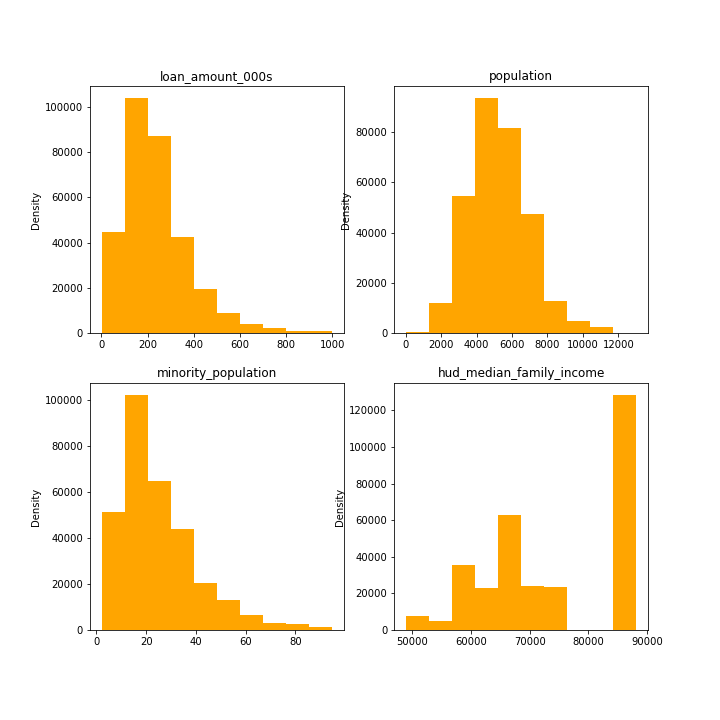
\includegraphics[scale = 0.5]{../plots/hmda_hist.png}
	
	The histograms are all very similarly shaped, and may be highly correlated. In particular the loan amount, population, and minority 
	populations seem to have very similar skewed right distributions. However, the data we have access to is yearly in nature, and the 
	variations in the Zillow data are monthly. For this reason we will only be using the Zillow data to for our time-series modeling. 

	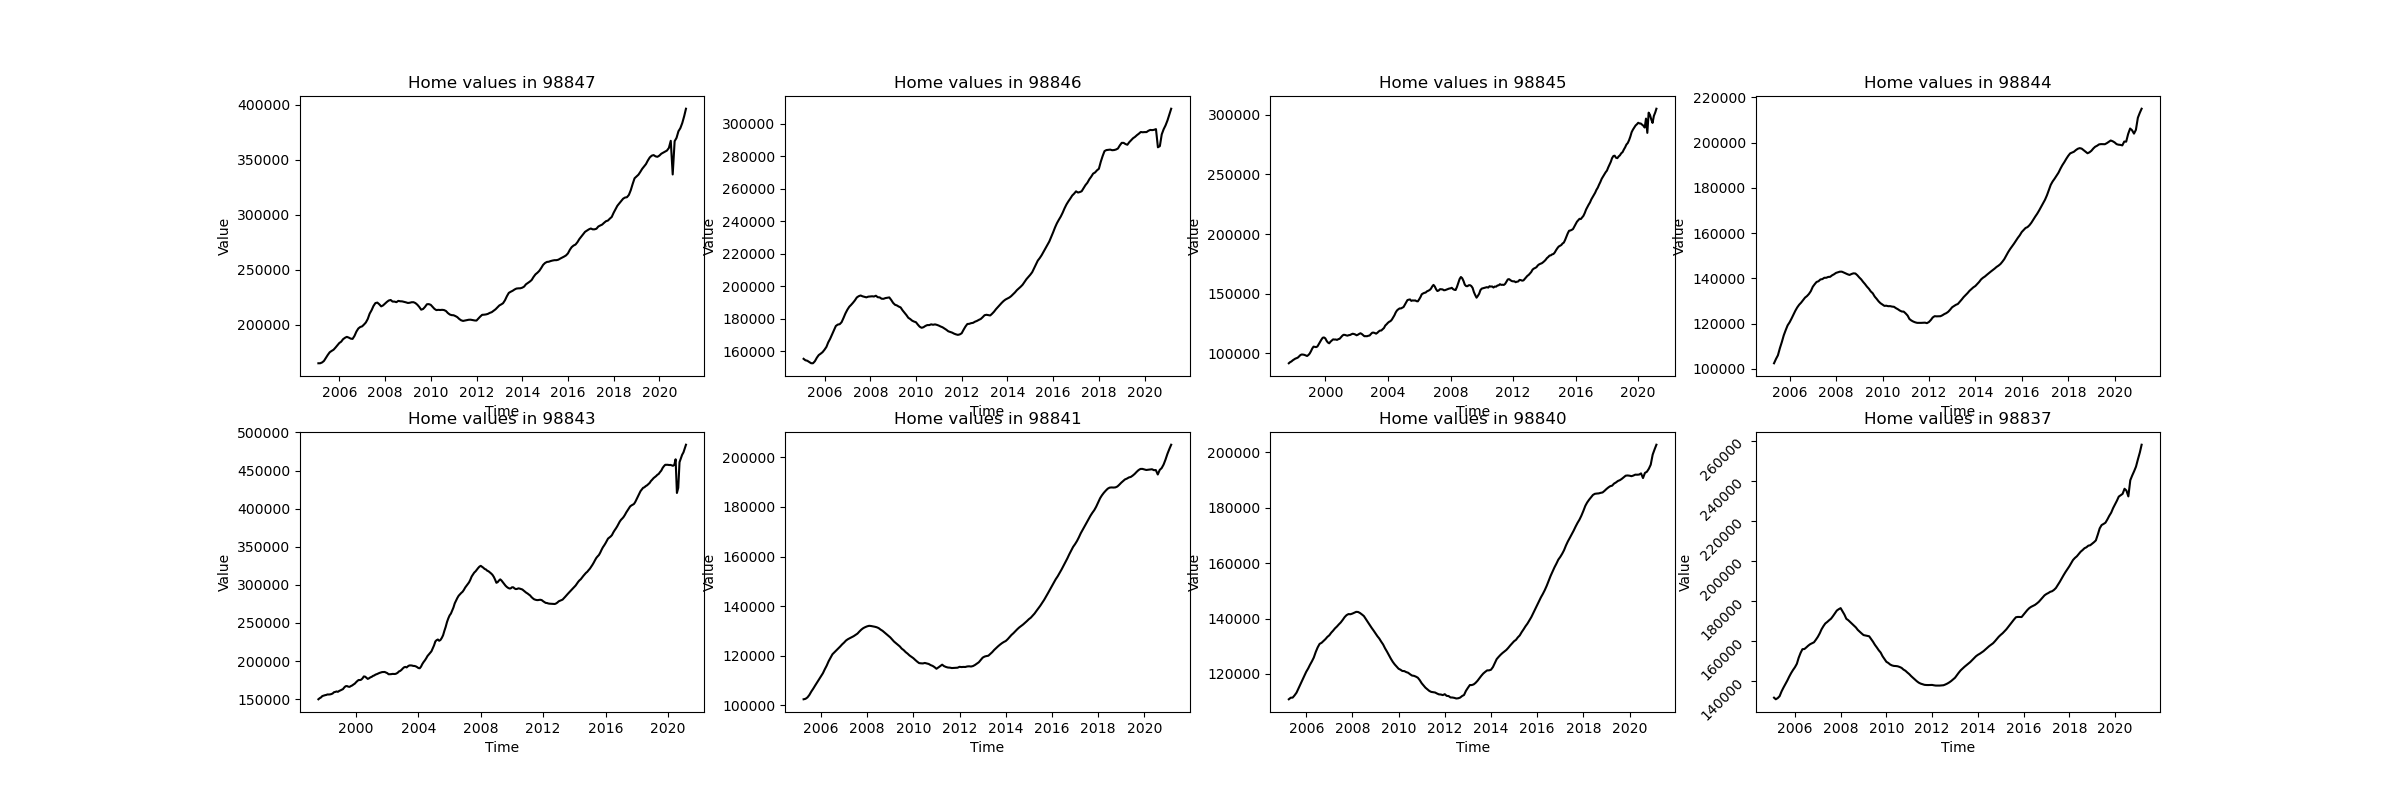
\includegraphics[scale=0.3]{../plots/zillow.png}
	
	As we can see from this sample of 
	
	\section{Modeling}
	\subsection{Auto-Regressive Model}
	Autoregression is a time series model that uses observations from previous time steps as input to a regression equation to predict the value at the next time step - resulting in accurate forecasts on a range of time series problems. \\
	
	A regression model, such as linear regression, models an output value based on a linear combination of input values. This technique can be used on time series where input variables are taken as observations at previous time steps, called lag variables. So, we can predict the value for the next time step (t+1) given the observations at the last two time steps (t-1 and t-2). \\
	
	Essentially, we are fitting data from the same input variable at previous time steps into the linear regression equation and that's why it's referred to as an autoregression (regression of self). \\
	
	Equation: X(t+1) = b0 + b1*X(t-1) + b2*X(t-2)\\
	
	Using the built-in plot in the Pandas library, we created a lag plot to visually check to see any auto-correlation in the time series data set. The figure below is the display of the lag plot. \\
	
	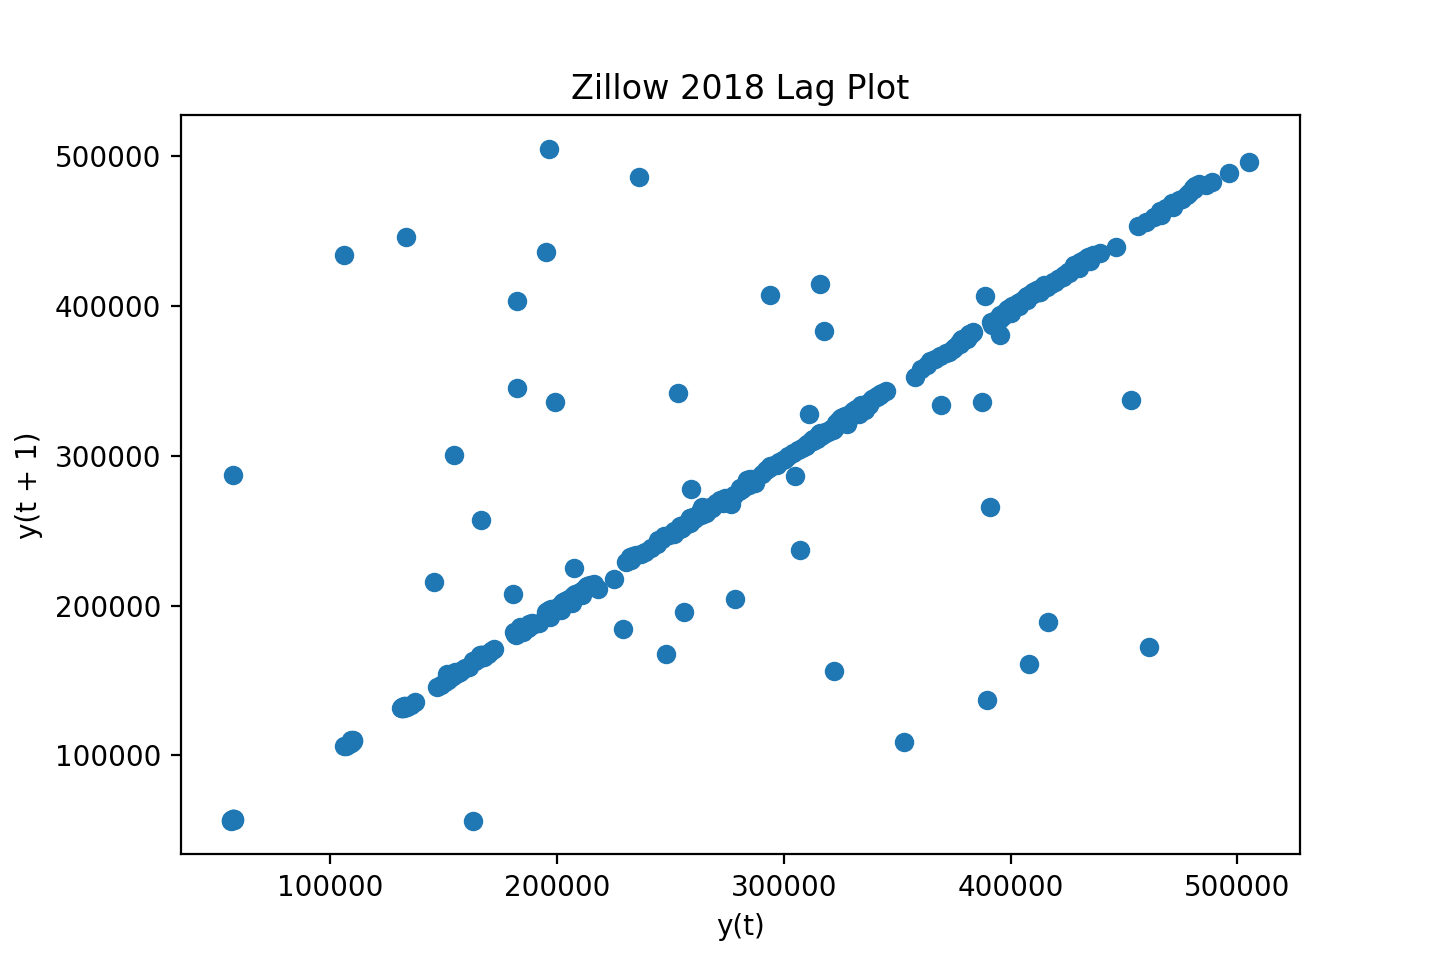
\includegraphics[scale = 0.2]{../plots/2018/zillow2018_lag.png} \\
	
	Auto-correlation is similar to correlation as they both describe the relationship between two variables. Auto-correlation calculates the relationship for time-series observations with the previous time steps or as mentioned before, lags. The linear pattern exhibited in the lag plot shows that the data are strongly non-random and further suggests that an autoregressive model might be appropriate. Strong positive correlation (0.901) between the observation and the lag=1 value. \\
	
	\begin{center}
    \begin{tabular}{ c c c }
     \smallskip & t-1 & t+1 \\ 
     t-1 & 1.000 & 0.901 \\  
     t+1 & 0.901 & 1.000    
    \end{tabular}
    \end{center} \\
	
	By plotting the correlation coefficient for each lag variable, we can get a good idea of which lag variables may be good candidates in our predictive model and see how the relationship between the observation and its historic values changes over time. \\
	
	The auto-correlation plot below is a 2D plot showing the lag number along the x-axis and the correlation coefficient value between -1 and 1 on the y-axis. The plot also includes solid and dashed lines that indicate the 95\% and 99\% confidence interval for the correlation values. Correlation values above these lines are more significant than those below the line, providing a threshold or cutoff for selecting more relevant lag values. \\
	
	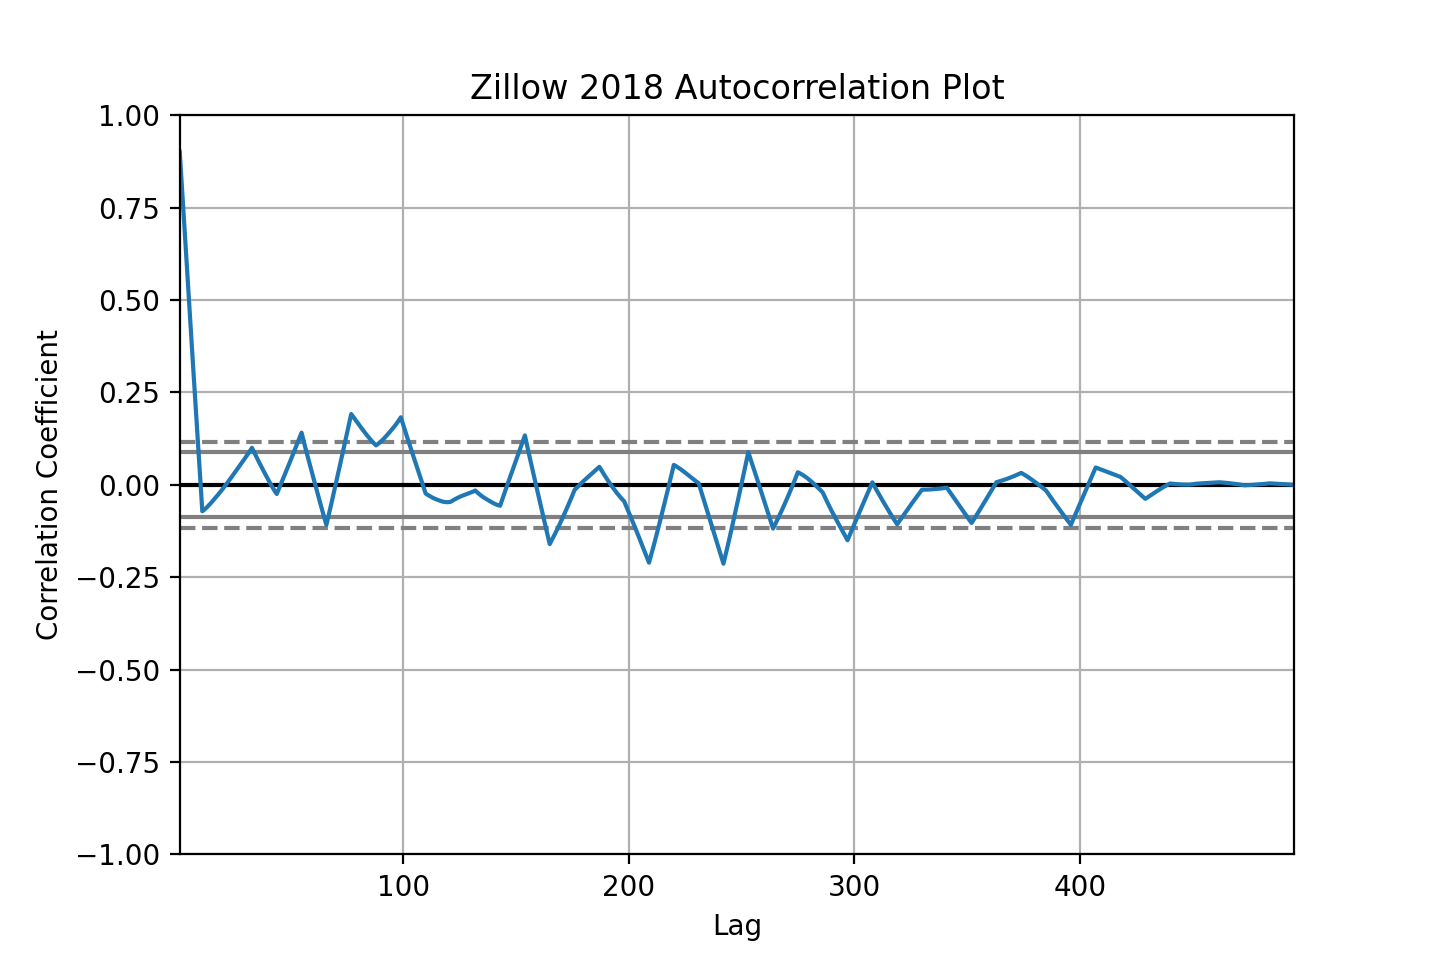
\includegraphics[scale = 0.2]{../plots/2018/zillow2018_autocorrelation1.png} \\
	
	The figure below is the same auto-correlation plot but with a limit of the lag variables evaluated to 31 for readability. The Confidence intervals can be seen as the shaded figures within the plot. By default the shaded figure cone is set to a 95\% confidence interval, suggesting that correlation values outside of this cone are very likely a correlation. \\
	
	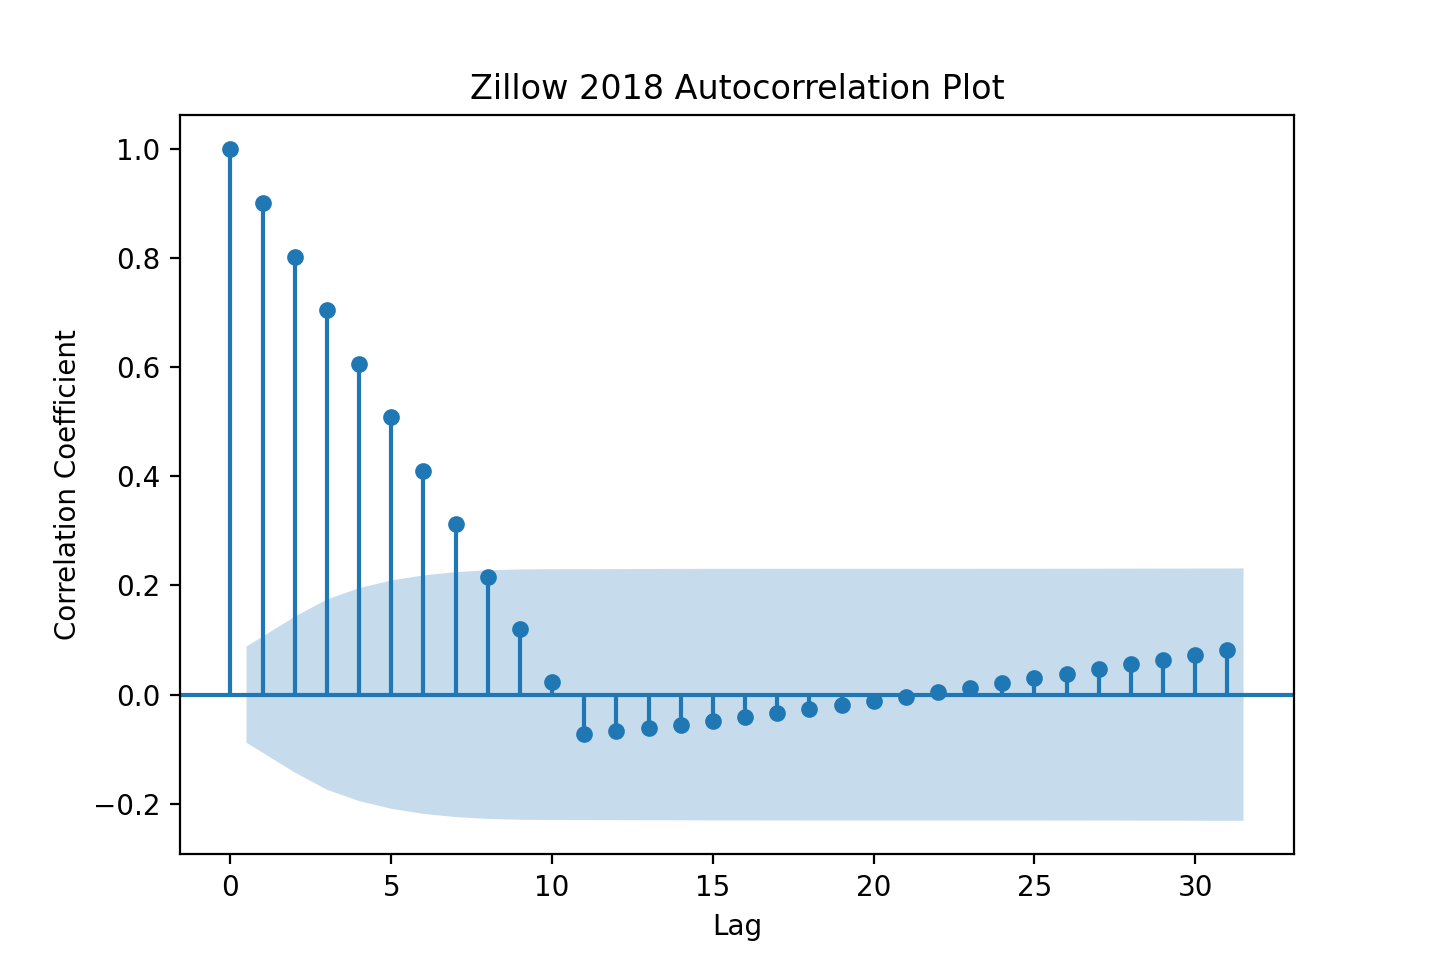
\includegraphics[scale = 0.2]{../plots/2018/zillow2018_autocorrelation2.png} \\
	
	The figure below is the baseline AR models and you can observe that it performs worse as the prediction range increases. \\
	
	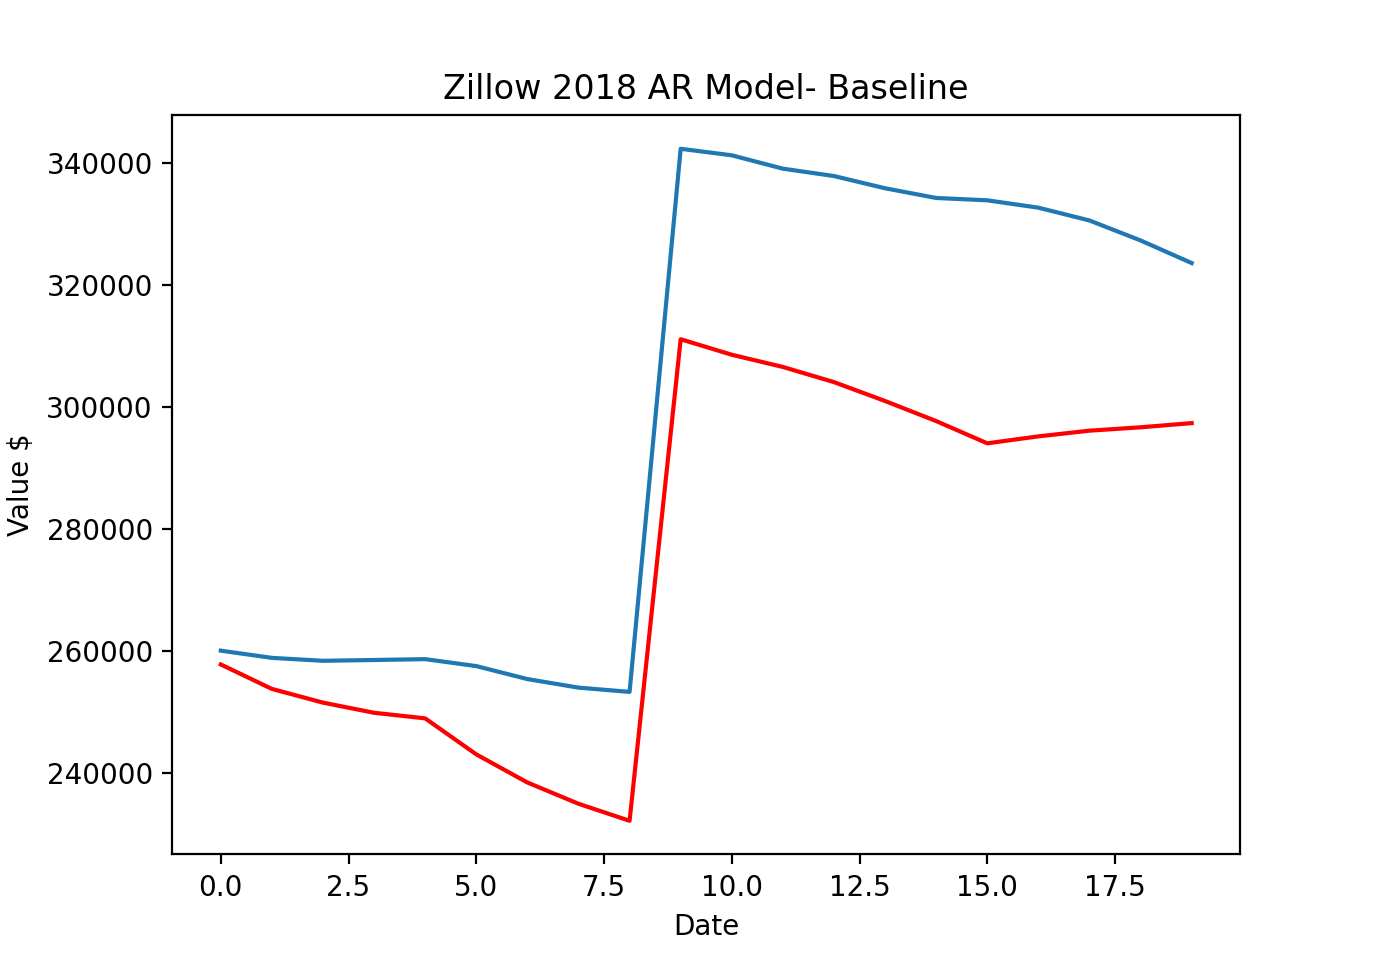
\includegraphics[scale = 0.2]{../plots/2018/zillow2018_AR-model-base20.png}
	\begin{center}
    \begin{tabular}{ c }
     AR Model 20 days forecast stats \\ 
     RMSE: 26,568.42 \\  
     Rsq: 0.527 \\
     MAPE: 0.076 \\
    \end{tabular}
    \end{center}
	
	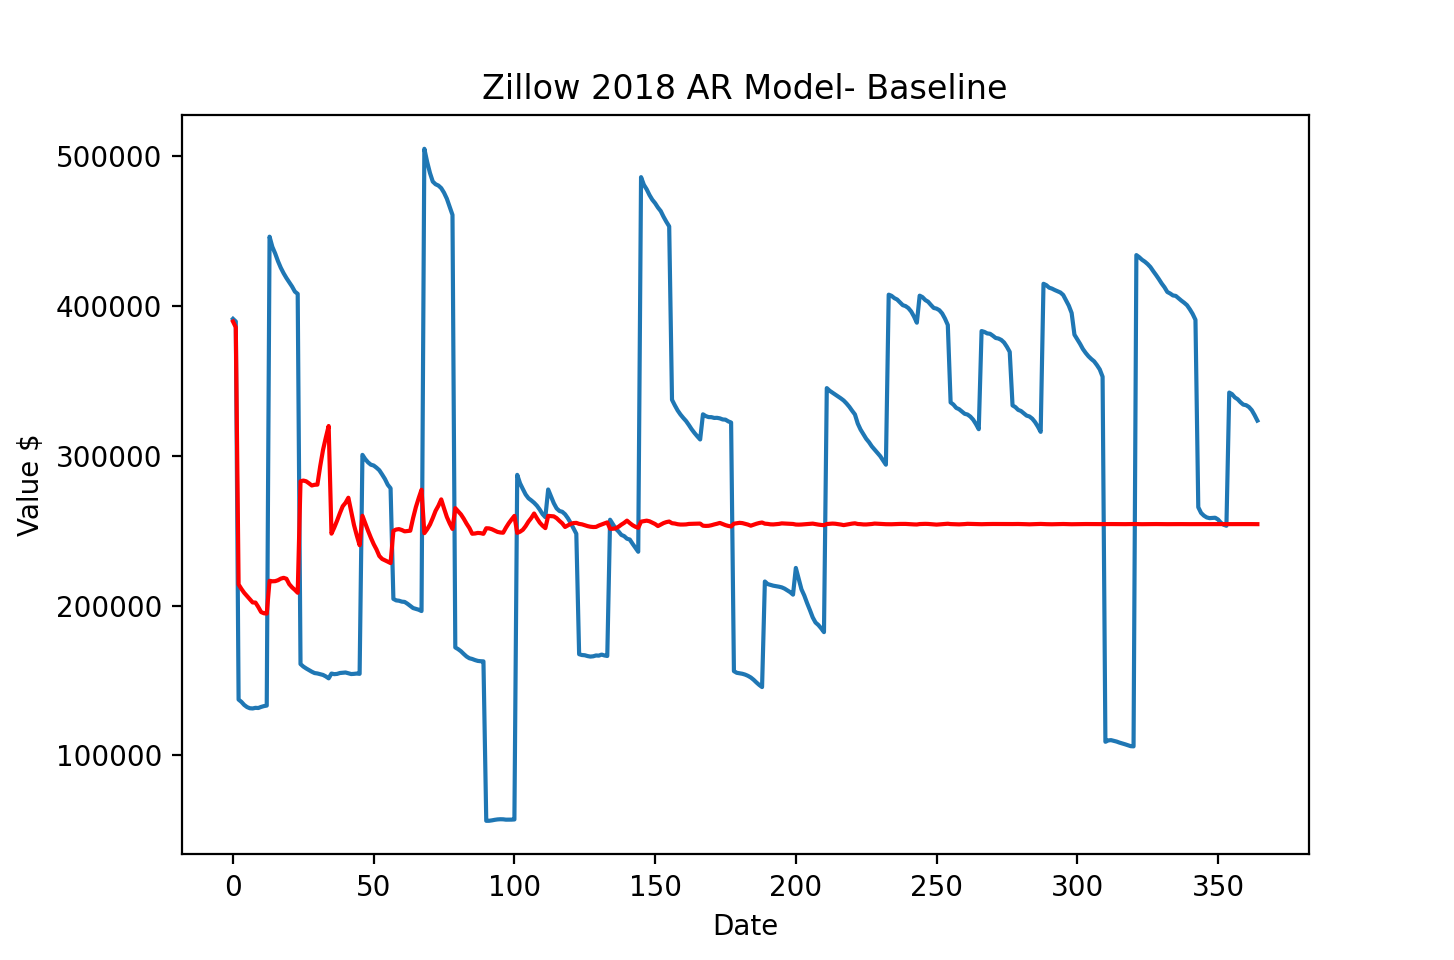
\includegraphics[scale = 0.2]{../plots/2018/zillow2018_AR-model-base365.png}
	\begin{center}
    \begin{tabular}{ c }
     AR Model 365 days forecast stats \\ 
     RMSE: 116,649.77 \\  
     Rsq: -0.114 \\
     MAPE: 0.454 \\
    \end{tabular}
    \end{center} 
	
	A method to tuning this model would be to use the learned coefficients and manually make predictions. This requires that the history of 29 prior observations be kept and that the coefficients to be retrieved from the model and used in the regression equation to come up with new forecasts. As you can see below the forecasts of model tuned is far more accurate and allows for a longer forecasting range. \\

	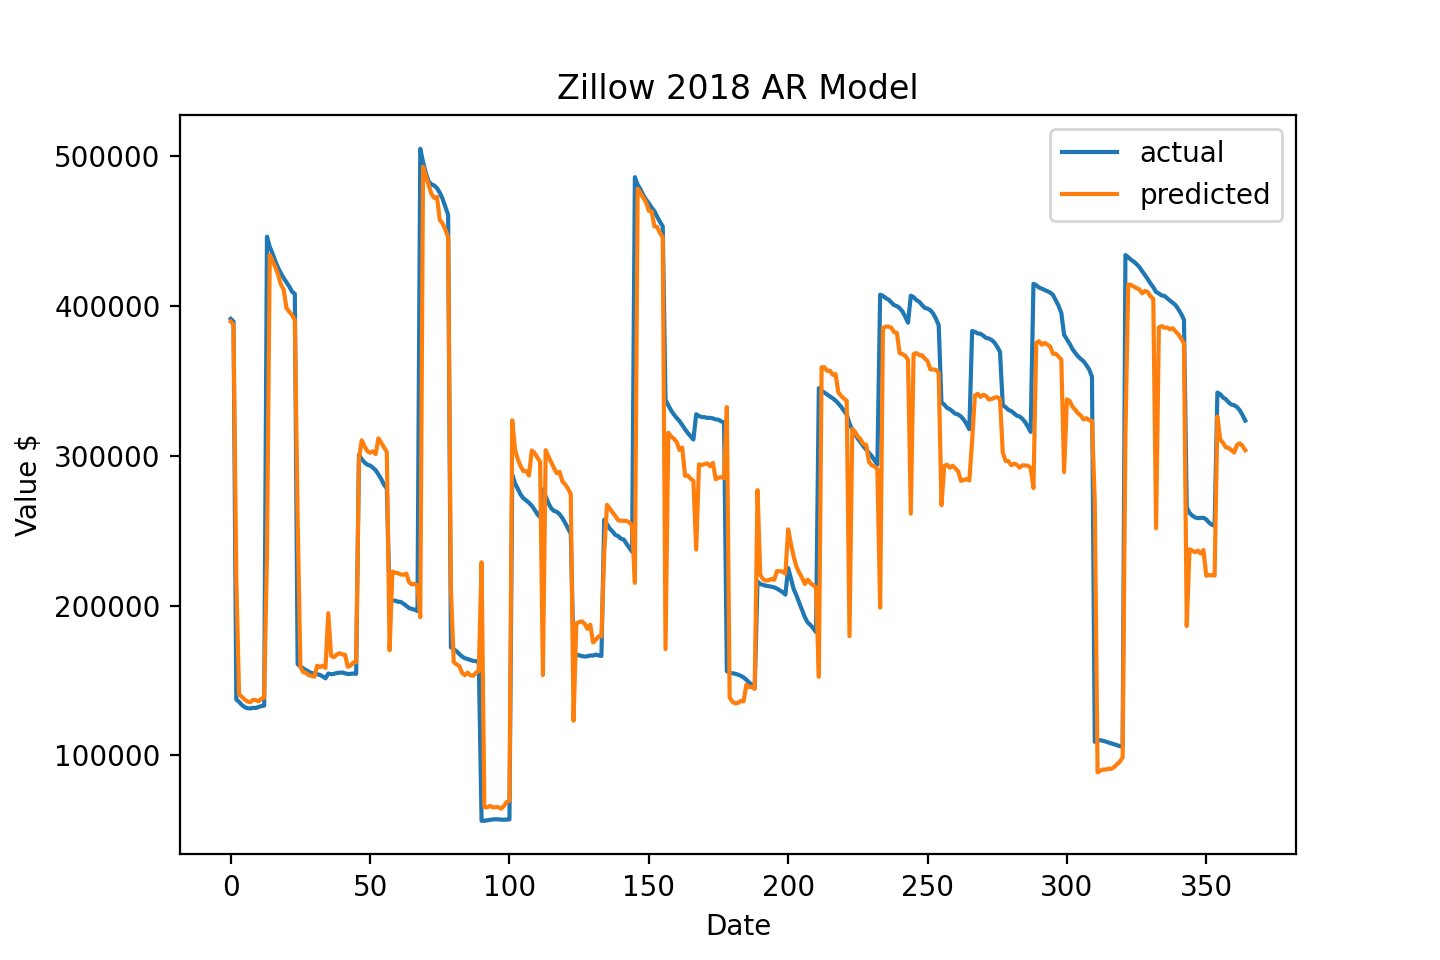
\includegraphics[scale = 0.2]{../plots/2018/zillow2018_AR-model.png}
	\begin{center}
    \begin{tabular}{ c }
     AR Tuned Model 365 days forecast stats \\ 
     RMSE: 45,571.047 \\  
     Rsq: 0.830 \\
     MAPE: 0.108 \\
    \end{tabular}
    \end{center}

    Tuning: The coefficients are provided in an array with the intercept term followed by the coefficients for each lag variable starting at t-1 to t-n. We simply need to use them in the right order on the history of observations, as follows: \\ yhat = b0 + b1*X1 + b2*X2 ... bn*Xn 

	\subsection{Seasonal Auto-Regressive Integrated Moving Average}
	The Seasonal Autoregressive Integrated Moving Average (SARIMA) method models the next step in the sequence as a linear function of the differenced observations, errors, differenced seasonal observations, and seasonal errors at prior time steps. \\
	
	The Seasonal Autoregressive Integrated Moving Average (SARIMA) method requires selecting hyperparameters for both the trend and seasonal elements of the series - so in total 7 parameters.\\
	
	Three trend elements:\\
    p: Trend autoregression order\\
    d: Trend difference order\\
    q: Trend moving average order\\

    Four seasonal elements:\\
    P: Seasonal autoregressive order\\
    D: Seasonal difference order\\
    Q: Seasonal moving average order\\
    m: Number of time steps for a single seasonal period\\

	An approach to tune the parameters is called grid search which is a suite of model configurations and discovers which configurations work. However, grid search requires extensive computing power. The code for grid search includes 7 nested for-loops which is about 70,000 models to iterate and test. Because of this reason, the performance of our SARIMA model presented is not the best model possible.\\
	
	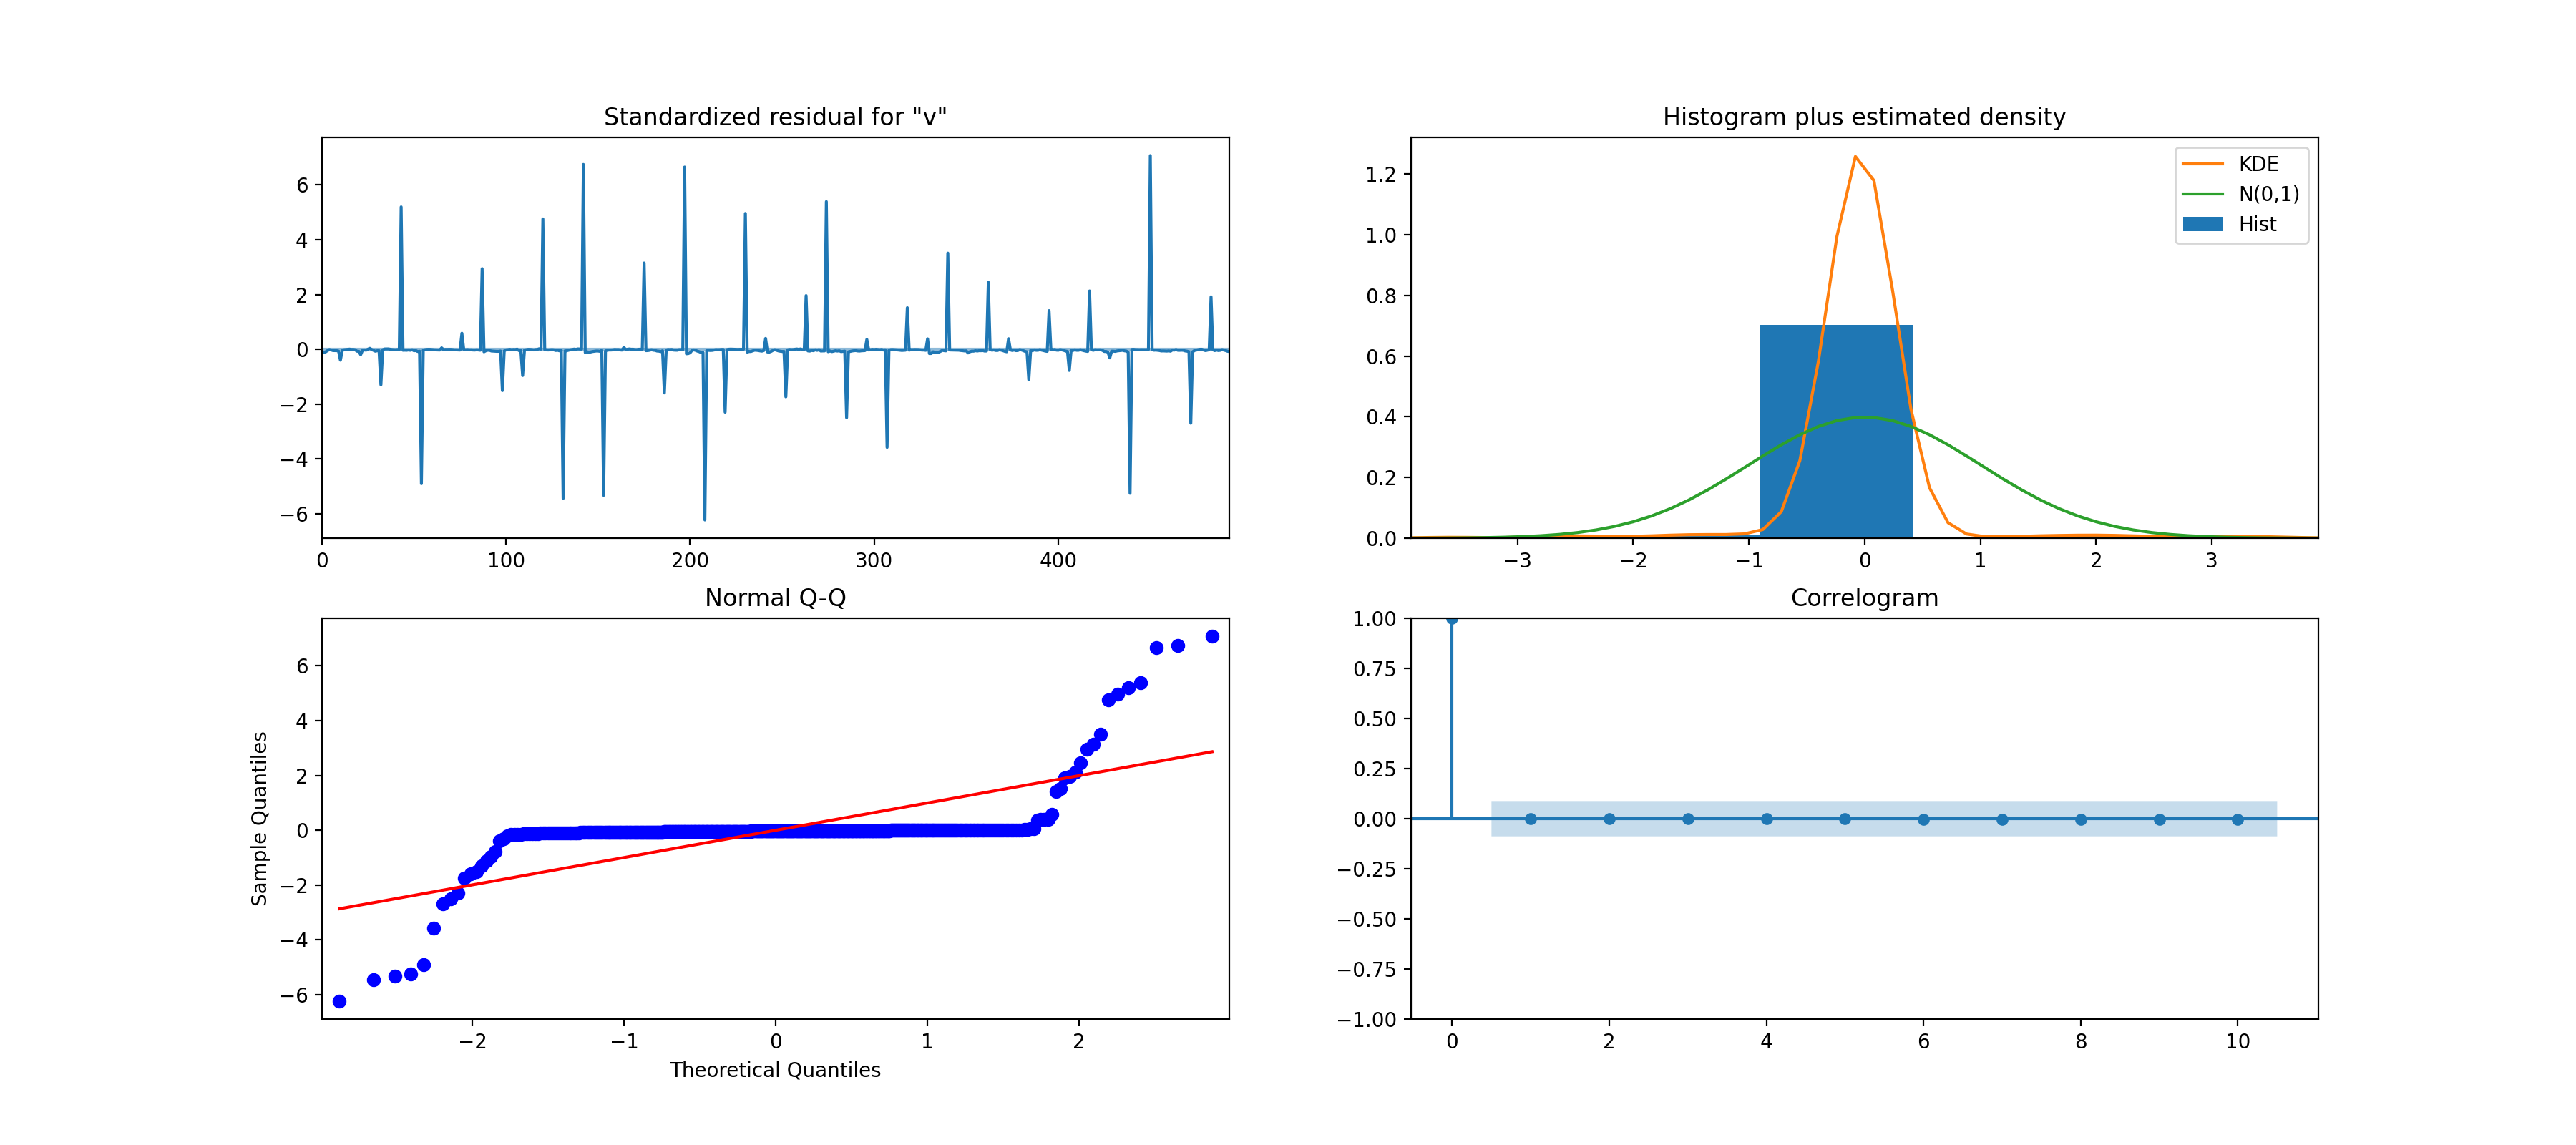
\includegraphics[scale = 0.2]{../plots/2018/zillow2018_SARIMA-model.png} \\
	
	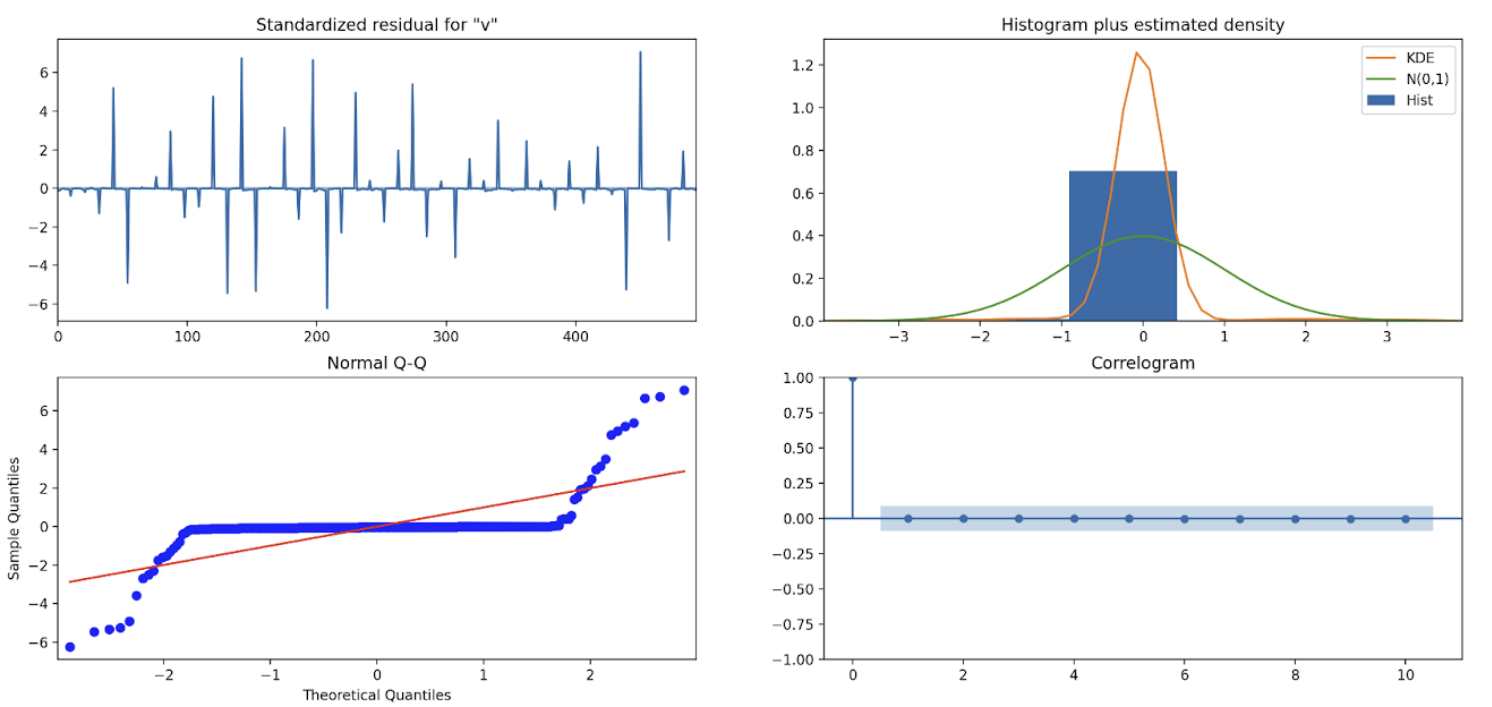
\includegraphics[scale = 0.2]{../plots/2018/zillow2018_SARIMA_stats1.png} \\
	
	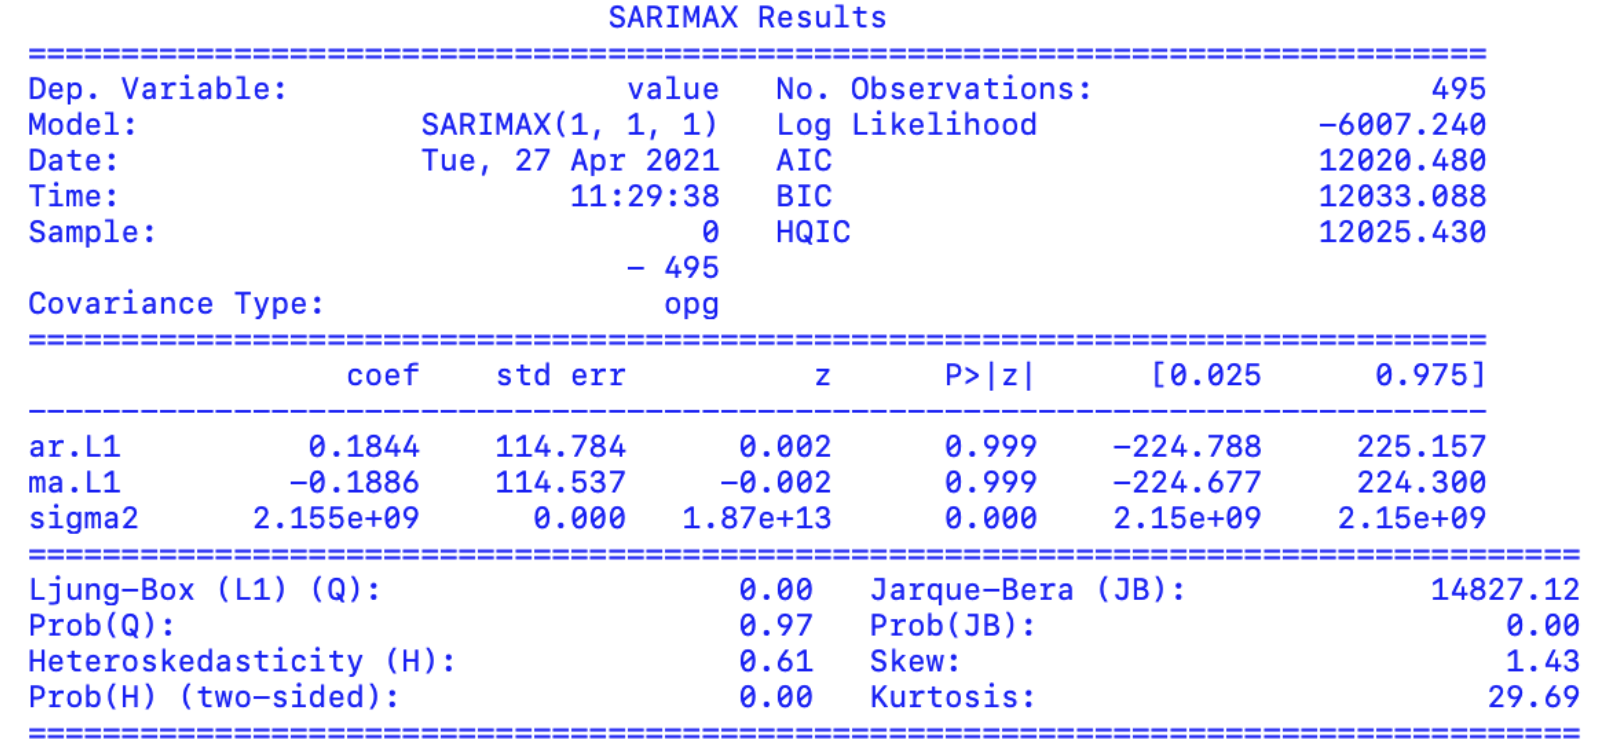
\includegraphics[scale = 0.2]{../plots/2018/zillow2018_SARIMA_stats2.png} \\
	\subsection{Gated Recurrent Unit RNN}
	
	The Gated Recurrent unit model requires inputs to be reshaped in a 3 dimensional input, where a particular value of at time $t_k$ 
	will be backed by m values ranging from $t_{k-m}$ to $t_{k-1}$ for every observation in the dataset. We used a GRU with 64 recurrent units 
	and the data was reshaped to use a look-back of 8 months as we found that was ideal. 
	
	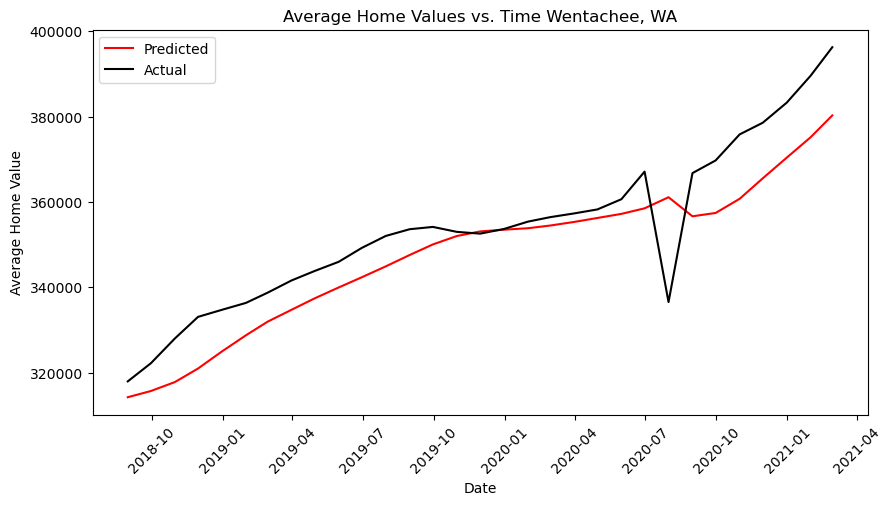
\includegraphics[scale = 0.5]{../plots/wentachee_1d_gru.png}
	
	Here were the results of the model: 
	
	\begin{itemize}
		\item $R^2$ - 0.69
		\item $RMSE$ - 9449.19
		\item $MAPE$ - 0.022
	\end{itemize}

	The GRU overall performed very well, and if wasn't for the black swan event that was the pandemic, the model would have performed even 
	better overall. We can see that the model is affected by the pandemic observation months after it happens because of the nature of the 
	time series. We could get around this problem by using a shorter look-back, but this may make the model too sensitive to observations that 
	come right before. 
	
	\subsection{Long Short-Term Memory}
	
	LSTM uses silimar shaped data as GRU, and maintains a control flow similar as an RNN. LSTM processes the data continuously as it grows 
	forward, while the data analyst is allowed to keep or forget the previous code. The analyst may choose to use the previous data through
	operations that can allow the LSTM to keep or forget information as an instruction.

	Graphs
	
	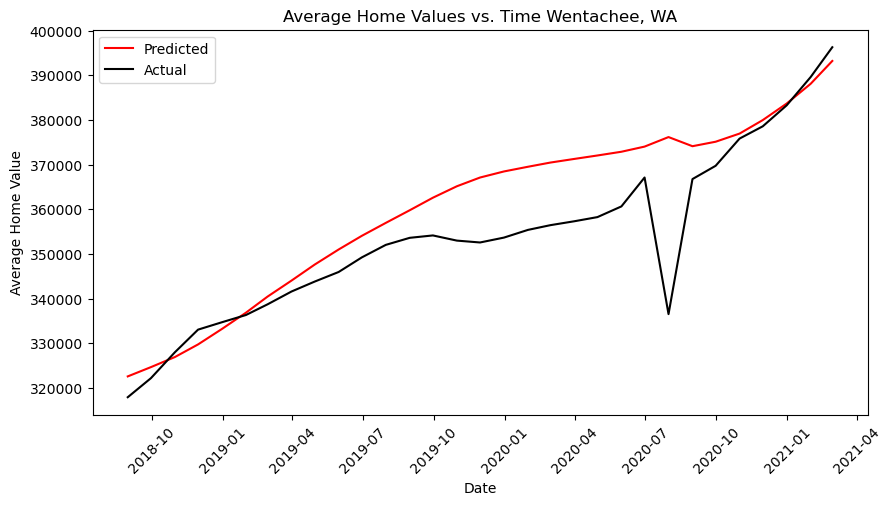
\includegraphics[scale = 0.4]{../plots/wentachee_1d_lstm.png}
	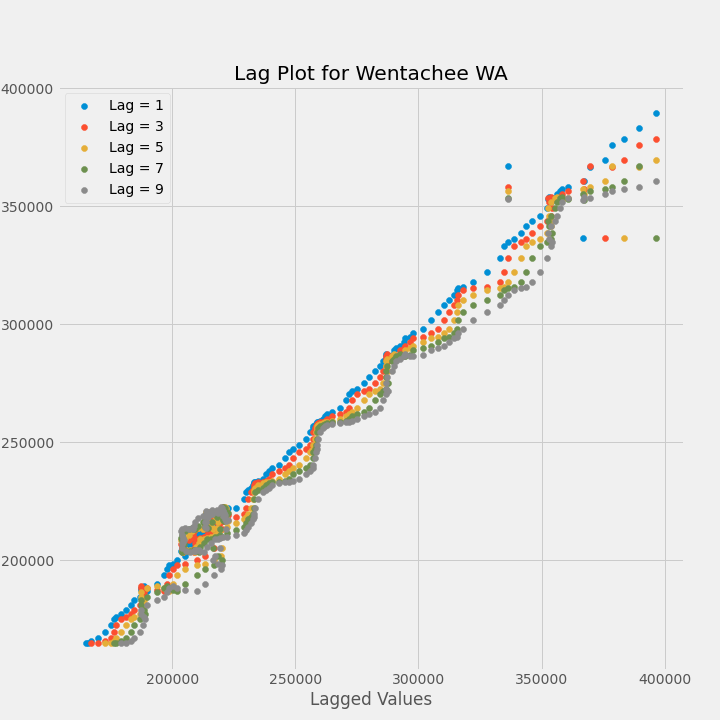
\includegraphics[scale = 0.4]{../plots/wentachee_lag.png}

	\subsection{Results}

	The LSTM gives us an accurate prediction that is slightly better than others. The R-Squared is the
	highest given of all three models (not including the autoregression). While the GRU model tended to
	underestimate, or rather undershoot the actual, the LSTM actually overshot it. The LSTM predicted
	higher numbers than the GRU, however both could not account for the dip in the housing market that 
	we believe was caused by the coronavirus pandemic. This is a reasonable assumption since these models
	cannot predict real world issues and events, only how a model should perform under the same previous
	circumstances. The lag plot given was also similar to the GRU, and gave farely accurate measurements
	as well.
	
	\section{Results \& Conclusion}
	
	Based on the results of our models, we believe that the best models in this case are the very simple auto-regressive models 
	simply because of the high performance and the simplistic nature of the data. We were able to accurately predict the 
	future housing prices solely on the basis of the previous values, and exogenous variables were not necessary.  

	
\end{document}
